\section{Algorithm}
%\textbf{Skeleton Partition.}
Let $M$ denote the mesh model, and let $S$ denote the Laplacian skeleton obtained via the algorithm provided in \cite{AuTCCL08}. We propose an algorithm for partitioning $M$ into a minimum set of \emph{disjoint} components, each of which can be fabricated by a 3D printer without using any support structure. Decomposing $S$ into two pieces can be done by duplicating a node $v$; while partitioning $M$ at node $v$ requires the determination of the position and normal of a cutting plane. To guarantee an aesthetical look on the resulting surface with shortest seams, we need a constraint to minimize the peripheral length of the cut in terms of the position and normal of the cutting plane. Note that the orientation of the cutting plane affects the printing direction and thus the shape of the subgraph while on the contrary, the shape of the subgraph constrains the orientation of the cutting plane. Hence, this is an essential \emph{chicken-and-egg} problem. {In addition, we need the assumption that the volume of the printing model should be within the working volume of a given 3{D} printer.}

%In addition, we also need to consider the printing volume limit, i.e., the volume of the printing model should be within the working volume of a given 3{D} printer.
To summarize, our objectives are the minimization of: (1) the number of partitioned components $N$ of the mesh model; (2) the total peripheral length of each cut $L_i$, i.e., $\Sigma L_i$. The constraints of the problem are as follows:

\begin{itemize}
\item (i) Each arc of the partitioned subgraph $H_i$ subtends to an axis by an angle of no larger than $\theta$, where $\theta$ is a printer-dependent parameter obtained from experiments. This guarantees that the corresponding mesh component is support-free during the printing process;

%\item (ii) As the directed arcs of $H_i$ are translated to a common origin, they form a fork (see Figure \ref{fig:cone}). Let $a$ and $b$ be the pair of farthest vectors in the fork, i.e., the angle between $a$ and $b$, denoted as $\alpha$, is the largest. Let the central ray of the minimum cone that encloses the fork be denoted as $r(H_i)$, then $r(H_i)$ is collinear with $a + b$. Then the feasible directions of printing $H_i$ without using any support is bounded by a solid cone centered at $r(H_i)$ with an apex angle of $2\theta - \alpha$ (Figure \ref{fig:cone}). Therefore, let $b(H_i)$ be the base cut of the mesh part that corresponds to the root of $H_i$ {(by base cut we mean the cutting boundary which adheres to the printing platform when the part is being printed, see Figure \ref{fig:ex1} (d))}, then $b(H_i)$ is orthogonal to some vector $\hat{e}$ in $cone(H_i)$. %This guarantees that the base can be placed on the 3D printing platform.
%    {\color{red}{Define the normal direction of each facet of a mesh component as pointing outwards. For a facet $c$ in a mesh component with base $b(H_i)$, we denote $n(c)$ as its normal direction. A cut on a shell model will result in two identical annuluses on the shell model. In order to guarantee support-free fabrication of any cut other than the base, each cut $c$ (a facet) in a mesh component with base $b(H_i)$ should satisfy the constraint that the angle between $n(c)$ and $n(b(H_i))$ is no smaller than $\pi/2-\theta$. Let $A(n(c),n(b(H_i)))$ denote the angle, then $A(n(c),n(b(H_i))) \geq \pi/2-\theta$. }} Since a cut separates the mesh into two parts, possibly sacrificing the angle constraint of the mesh part corresponding to a subgraph adjacent to $H_i$, an additional cut respecting the angle constraint of the adjacent subgraph may be required. Detailed steps for addressing this issue is given in the section for Mesh Partition below.

\item (ii) The base of a printing model should be large enough to gather sticky force from the building platform, such that the model is not deformed during the building process. Formally, let $area(b(H_i))$ denote the area of the base of the mesh component corresponding to $H_i$, which is approximately equal to the peripheral length of the base times the thickness of the shell. let $\tau$ be a user-defined threshold value, then we have $b(H_i) \geq \tau$. Here $\tau$ can be determined empirically;

\item Finally, (iii) Each cut partitions a single subgraph.

\end{itemize}

\begin{figure}[t]
  \centering
  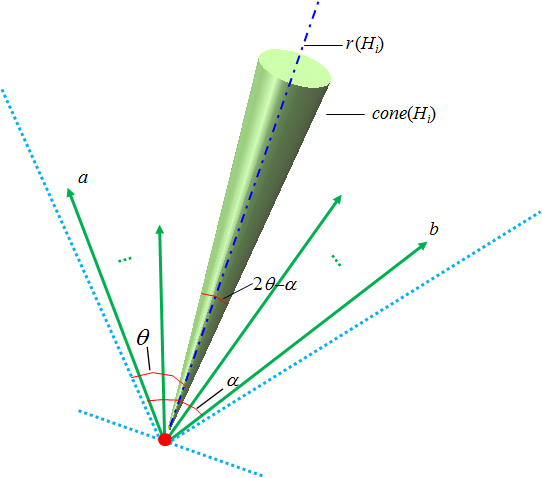
\includegraphics[width=0.7\linewidth]{figs/cone.png}
  \caption{\label{fig:cone}%
           Illustration of $r(H_i)$ and $cone(H_i)$.}
\end{figure}


We have the following optimization system:
\begin{equation*}
\begin{aligned}
& \underset{x}{\text{minimize}} \quad N \quad \text{and} \quad \sum_{i=1}^N{L_i},
\quad \text{subject to:} \\
& A(e, r(H_i)) \leq \theta, \; i = 1, \ldots, m, \forall e \in H_i, & (1)\\
& b(H_i) \bot \hat{e}, \exists \hat{e} \in cone(H_i), & (2)\\
%& A(n(c),n(b(H_i))) \geq \pi/2-\theta, & (3)\\
& area(b(H_i)) \geq \tau, & (3)\\
& cut \cap S = cut \cap H_i, cut \in \{b(H_i), c\}  & (4)
\end{aligned}
\end{equation*}
where all $H_i$-s constitute a partition of the original graph. A direct exploration of all possible partitions over the graph $G$ could quickly leads to exponential complexity. The key here is to quickly find potential good partitions in a way that subsequent exploration of the graph is limited to those which leads to a less value of the optimization function. We employ a randomized Monte Carlo algorithm detailed below.

We separate the minimization of the two target terms sequentially, i.e., the number of mesh components and the total cutting length. In the following, we shall discuss how the skeleton and mesh are partitioned in details.

\textbf{Skeleton Partition.} {{To minimize the number of mesh components, we need to provide a proper set of partitioned subgraphs from $S$.}}
For this purpose, we use a randomized exploration strategy, but give a higher probability to explore the graph broadly. In particular, assume that we are given a function $Trim\_BFS(v, G, \theta)$ which traverses $G$ from $v$ in a breath-first search manner to progressively collect arcs which satisfy constraint (i); and a function $MeshPartition(U , M)$ that decomposes $M$ based on the set of partitioned subgraphs $U$, and returns a partition of $M$, denoted as $M^{'}$, and the number of cuts $N$. Algorithm \ref{alg:Framwork} sketches the idea of the skeleton decomposition {{by minimizing $N$}}. The main idea is to randomly search for candidate subgraphs using Monte Carlo Method, which randomly chooses a node of $G$ to start traversing and randomly grows the subgraph while paying attention to the aforementioned constraints.

\begin{algorithm}
\caption{$Skeleton\_Mesh\_Decomposition(S, M)$}
\label{alg:Framwork}
\begin{algorithmic}[1]
\REQUIRE~
The Laplacian skeleton $S$ and mesh model $M$.
\ENSURE~
The decomposition of $M$ into the least pieces of components that are free of support.

%; a partition of $M$ based on $T$ that satisfies constraint (2-4)
\STATE $M_{opt} = \emptyset$; $min = \inf$; $count$ = 0; $max\_iter$ = a user defined large constant;
\WHILE {$count < max\_iter$}
\STATE  $U= \emptyset$;
\STATE  $X= S$;
\WHILE {$S\neq \emptyset$}
%\FOR{$i=1$; $i<|| S ||$; $i++$ }
\WHILE{a random node $v \in S $ }
\STATE $H = Trim\_BFS(v, X, \theta)$;
\STATE $X = X / H$;
\STATE $U = U \cup H$;
\ENDWHILE
\STATE $(M^{'}, N) = MeshPartition(U , M)$;
\IF {$N < min$}
\STATE  $min = N$;
\STATE  $M_{opt} = M^{'}$;
\ENDIF
\ENDWHILE
\STATE $count =count + 1$;
\ENDWHILE
\RETURN  $M_{opt}$;
\label{code:fram:select} \\
%\STATE call function $Mesh\_Decomposition(M, T)$;
\end{algorithmic}
\end{algorithm}

\begin{figure}[tbp]
  \centering
  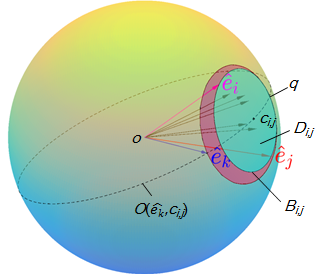
\includegraphics[width=0.7\linewidth]{figs/take_arc.png}
  \caption{\label{fig:sphere}%
           Illustration of unit vectors, unit sphere, spherical disks, and the determination of taking a new edge in $Trim\_BFS$.}
\end{figure}

Next we shall show how $Trim\_BFS(v, G, \theta)$ works to find a locally maximal subgraph starting at $v$ that satisfies the angle constraint. Let $H$ be the current subgraph obtained so far. When an arc $e$ of $G$ is visited, we need to determine whether it should be included into $H$. If the start of each outgoing arc of $H$ is moved to a common origin, then the arcs form a fork of rays (Figure \ref{fig:sphere}). A naive method for judging whether $e$ should be included is to move the start of $e$ to the origin of the fork, and compute the angle between $e$ and each arc of the fork, $e$ is included if the maximum angle between $e$ and each arc of the fork does not exceed 2$\theta$. However, this would lead to $O(n^{2})$ time complexity of $Trim\_BFS(v, G, \theta)$, where $n$ is the size of $G$. To speed up this process, we keep the pair of vectors which form the largest angle and judge whether a new vector expands the angle of the fork. See Figure \ref{fig:sphere}, let $\hat{e_i}$  and $\hat{e_j}$ be the units of these two vectors obtained so far. For simplicity, we denoted by $F( \hat{e_i}, \hat{e_j} )$ the fork with the starts of all unit vectors converging at the origin of the coordinate frame, where $\hat{e_i}$  and  $\hat{e_j}$  are the pair of unit vectors that form the largest angle in the fork. Let $\hat{e_k}$  be the unit of a new vector to be processed next, if $\hat{e_k}$ penetrates through the blue circle, then no change needs to be made to the fork; otherwise, let $D_{i,j}$ denote the spherical disk that passes through the endpoints of $\hat{e_i}$  and $\hat{e_j}$ whose central axis is collinear with $\hat{e_i}$  + $\hat{e_j}$, let $c_{i,j}$ be the center of $D_{i,j}$, let $B_{i,j}$ be the boundary circle of $D_{i,j}$. The circle passing through $\hat{e_k}$  and $c_{i,j}$, denoted as $O( \hat{e_k}, c_{i,j})$, intersects  $B_{i,j}$ at two points, $q$ and the endpoint of $\hat{e_k}$, then $\overrightarrow{oq}$ and $\hat{e_k}$ are the two extreme vectors that to be used in the next iteration. To summarize, a new arc $e_k$ is taken by $Trim\_BFS$ if and only if one of the following two conditions is met:
(1) the angle between $\overrightarrow{oc_{i,j}}$ and $\hat{e_k}$, denoted as $A(\overrightarrow{oc_{i,j}}, \hat{e_k})$, satisfies  $A(\overrightarrow{oc_{i,j}}, \hat{e_k}) \leq A(\overrightarrow{oc_{i,j}}, \hat{e_i})$;
(2) $A(\overrightarrow{oq}, \hat{e_k})  \leq  2\theta$, where $q = O( \hat{e_k}, c_{i,j}) \cap B_{i,j}$.


\begin{algorithm}[t]
\caption{Algorithm: $Trim\_BFS(v, S,\theta)$}
\label{alg:trim}
\begin{algorithmic}[1]
\REQUIRE~
A node $v$ of Laplacian skeleton $S$, an angular value $\theta$.
\ENSURE~
 %A maximal subgraph $H$ rooted at $v$ and its corresponding mesh component that meet the constraints $(Eq.1-4)$.
 A subgraph $H$ rooted at $v$ that meets constraint (1).
\STATE starting from $v$, initialize F($\hat{e_i}$, $\hat{e_j}$); $H = \emptyset $;
\WHILE  {a random arc $e_k$ of $S$ visited by BFS}
  \IF  {$A(\overrightarrow{oc_{i,j}},  \hat{e_k}) \leq A(\overrightarrow{oc_{i,j}},  \hat{e_i})$}
  \STATE  $H = H \cup \{e_k\}$;
  \ELSIF {$A(\overrightarrow{oq},  \hat{e_k}) \leq  2\theta$}
  \STATE $q = O( \hat{e_k}, c_{i,j}) \cap B_{i,j}$;
%  \IF  {$A(\overrightarrow{oq},  \hat{e_k}) \leq \pi- 2\theta$}
  \STATE  $\hat{e_i}=  \hat{e_k}$;
  \STATE $\hat{e_j} =  \overrightarrow{oq}$;
  \STATE  update $B_{i,j}$ and $c_{i,j}$;
  \STATE  $H = H \cup \{e_k\}$;
  \ENDIF
\ENDWHILE
%\STATE  call the cutting scheme for $M$;
%\STATE  $M= M/M_H$;
\label{code:fram:select} \\
%\RETURN  $H$ and $M_H$;
\RETURN  $H$;
\end{algorithmic}
\end{algorithm}

Algorithm \ref{alg:trim} demonstrates the growing process. Since the order of the chosen arcs influences the shape of the final BFS subgraph, in line $2$, the BFS process randomly chooses an arc incident to $v$ to proceed on. In order to guarantee a greater chance of converging to the optimal result in a short time, we refine Algorithm \ref{alg:trim} by inducing probabilities of choosing each arc of $S$. We denote this improved version of Algorithm \ref{alg:trim} as \textbf{$Trim\_BFS\_II$}. The main idea of $Trim\_BFS\_II$ is as follows.
We apply a training-and-learning procedure for the first $k$ (say $1000$) runs. Formally, let $n_v$ be the number of times an arc is chosen as the exit arc when node $v$ is visited. Given the data of the first $k$ runs, when a node $v$ is visited, the probability of choosing an arc $e$ as exit in the subsequent runs is, $P(v, e) = n_v/k$.

%To further speed up the process of $Trim\_BFS$, we assign a mark that stores the minimum number of subgraphs obtained so far, such that the current branching can be terminated if its output number of subgraphs is larger than the mark.

Further, as $Trim\_BFS\_II$ is greedy, the growth is towards a local maximal subgraph that satisfies the angle constraints, the resulting partition of Algorithm \ref{alg:Framwork} might not be a global optimum. In order to ensure more possibilities to find a global optimum, we set a probability-based scheme to terminate the growing of a subgraph. The probability to terminate the growing is set to $r/n$, where $r$ is the size of the current subgraph and $n$ is the size of $G$. This gives high probability for $Trim\_BFS\_II$ to grow in larger sizes while rising the probability of exploring subgraphs of smaller sizes. We implemented it using rejection sampling.

%Since the traversing process assigns a specific direction to each arc that was originally undirected in $S$, it is not obvious whether the angle constraint is satisfied, To clarify this, we provide the following lemma.


%\begin{figure}[t]
%  \centering
%  \mbox{} \hfill
%  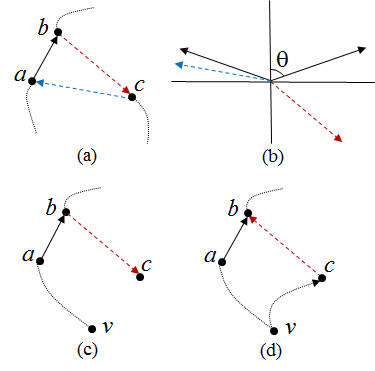
\includegraphics[width=0.4\textwidth]{figs/proof.png}
%  \caption{\label{fig:proof}%
%           Illustration of taking a directed arc into a maximal subgraph by $Trim\_BFS$.}
%\end{figure}



%\emph{Lemma 1}: $H = Trim\_BFS(v, G, \theta)$ is a maximal subgraph of $G$ that satisfies the angle constraint, i.e., each arc of $H$ subtends to an axis by an angle of no larger than $\theta$.


%\emph{Proof}: Suppose to the contrary that $H$ violates the angle constraint, there exists a directed arc that does not satisfy the angle constraint. For example, arc $\overrightarrow{ca}$ or arc $\overrightarrow{bc}$ in Figure \ref{fig:proof}. Such case is impossible as Line $3$ and Line $6$ of function $Trim\_BFS$ excludes any directed arc that violates the angle constraint of no larger than $\theta$ with respect to the (virtual) central axis.It remains to prove that $H$ is maximal, i.e., the largest graph rooted at $v$ that covers all the arcs that satisfies the angle constraint. Suppose that this is not true, there must exist an arc that was mistakenly discarded due to the direction in which the arc is traversed. Let $(b, c)$ be one of such arcs, as illustrated in Figure \ref{fig:proof}(a). When the arc is directed from $b$ to $c$, it is not included as it violates the angle constraint, but can be included if the arc directed from $c$ to $b$. We shall prove in a case-by-case basis. If $c$ is not reachable from $v$ via a directed path passing through $b$ (Figure \ref{fig:proof} (c)), then $c$ is only reachable from $b$, arc $bc$ should not be included and line 6 of Function $Trim\_BFS$ correctly handle this case. Otherwise, $c$ is reachable from $v$ via a directed path without passing through $b$ (Figure \ref{fig:proof} (d)). As $c$ is visited, by Line 2 of Function $Trim\_BFS$, each arc leaving $c$ is considered, and $\overrightarrow{cb}$ is correctly included into $H$. This completes the proof.



\begin{figure}[t]
  \centering
  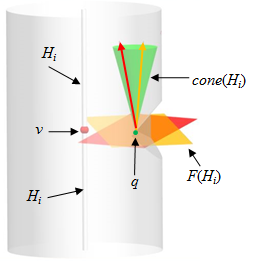
\includegraphics[width=0.3\textwidth]{figs/cone-fillet.png}
  \caption{\label{fig:fillets}%
           Illustration of a cone and its corresponding fillets, where two cutting planes in $F(H_i)$ and their associated vectors in $cone(H_i)$ are marked by distinct colors.}
\end{figure}


\textbf{Mesh Partition.}
{{In the following section, we shall describe how $MeshPartition(U , M)$ works as a cut is required around a skeleton node $v$. Here the pseudocode is omitted for brevity.}}
The skeleton partition returns a set of nodes where the mesh partition should occur, in particular, the cutting plane should be in the vicinity of each node $v$ incident to at least two distinct subgraphs. We need to determine the exact positions and orientations of the cutting planes. For each node $v$ that is incident to at least two distinct subgraphs $H_i$ and $H_j$, we process it using the following cutting scheme.
Refer to Figure \ref{fig:fillets}, at the position of node $v$, we want to find a surface vertex $q \in M$ around $v$ through which the cutting plane should pass, while the cutting length is minimized. Let us denote the set of all planes which pass through a surface vertex $p$ and are orthogonal to vectors in $cone(H_i)$ (originated from $p$)  as $F(H_i)$, which we term as a \emph{fillet}. If the node $v$ is incident to two subgraphs $H_i$ and $H_j$, we have two plane sets $F(H_i)$ and $F(H_j)$ at point $p$, respectively. Depending on the position of $p$, we have the following two cases. \emph{Case (i)}: $F(H_i) \cap F(H_j) \neq \emptyset$. In this case, we shall randomly sample a set of cutting planes from $F(H_i) \cap F(H_j)$, and determine the one achieving the minimum cutting length; \emph{Case (ii):} $F(H_i) \cap F(H_j) = \emptyset$. In this case, two cuts $c_1$ and $c_2$ are required in order to separate the mesh into support-free subparts. However, care must be taken as the angle between $c_1$ and $c_2$ should be constrained by $A(c_1, c_2) \leq \pi/2-\theta$. If this constraint is violated, one more cut in between $c_1$ and $c_2$ is required. Meanwhile, the base of each partitioned component should be no less than $\tau$. If any of the constraint is not satisfied, we shall translate the fillets along the printing direction in an opposite sense until the constraints are satisfied.

\begin{figure}[tbp]
  \centering
  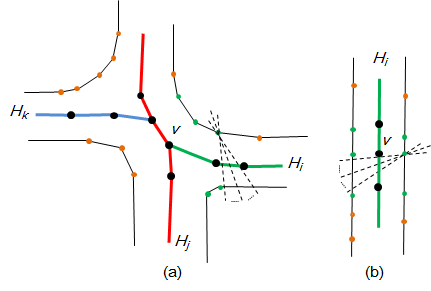
\includegraphics[width=0.5\textwidth]{figs/forward_tracing.png}
  \caption{\label{fig:forward_tracing}%
           2D illustration of $R(v)$ and the cuts, all vertices in $R(v)$ are shown in green, and the cuts associated with a vertex are shown in dashed lines:(a) the case of cuts around concave points; (b) the case of cuts on a cylindrical part.}
\end{figure}

In either case, a cut that nicely follows the geometry features is demanded in order to preserve aesthetic appearance in the final assembled object. We exploit shape concavity to look for a good cut as indicated by minima rule \cite{hoffman1984parts,hoffman1997salience}. However, the positions of the skeleton nodes may not locally reflect the geometric features such as concave areas on the mesh surface, therefore they are insufficient for a nice partition of the mesh. To compensate this, we exploit the concave vertices of the mesh that are incident to the skeleton nodes and take those that significantly concave into a candidate set of pivots for the cuts. More precisely, let $R(v)$ be the set of concave vertices on $M$ that are incident to $v$ during the Laplacian shrinking process \cite{AuTCCL08}, we truncate $R(v)$ such that the insignificant concave vertices are removed away. Here, given a vertex $v_i$ and any of its neighbor $v_j$, $v_i$ is concave if $(v_i - v_j)(n_j - n_i)$ is nonnegative, the significance of a concave vertex, denoted as $\tau_i$, can be quantified as the magnitude of $(v_i - v_j)(n_j - n_i)$ \cite{au2012mesh}. We collect vertices whose $\tau_i$ is greater than a threshold $\delta$.
%See Figure \ref{fig:fillets}(c-d), for each vertex in $R(v)$, we shall process a pair of fillets as done for vertex $p$ above.
Next, we proceed to find a cutting plane around $v$. We first extend $R(v)$ by merging each $R(u)$ into it, where $u$ is an adjacent node of $v$ in $S$. Given all concave vertices in the new $R(v)$, each vertex defines a set of feasible cutting planes in accordance to its $fillet$. By feasible we require that a cutting plane does not cut through any other subgraph except for $H_i$. We then exhaustively go through all feasible cutting planes and find the one whose cutting length is minimum. In case of a cylindrical part that does not merit good concaveness, we reduce the threshold value $\delta$ by half and repeat the procedure until a feasible cutting plane with minimum length is found. Figure \ref{fig:forward_tracing} illustrates the process.
%Particularly, if $v$ is a leaf node that is merely neighbored to a single node $w$ in subgraph $H_i$, then the separation of the mesh component corresponding to $H_i$ may not be feasible if merely $R(v)$ is used, this is because the position of $v$ is chosen irrespective of the geometric features of the mesh. To separate the mesh component of $H_i$, we process arc $vw$ as follows: Given a user-defined threshold value $\delta$, if $| vw | \leq \delta$, then $R(v)$ is extended to contain the concave vertices of $M$ that are incident to $w$. On the other hand, if $| vw | > \delta$, then a partition of the arc $vw$ by an interval of $\delta$ is carried out. Subsequently, for each node along arc $vw$, the above scheme for processing node $v$ is exploited, see Figure \ref{fig:forward_tracing}. In this process, the tracing of the nodes along $vw$ stops as a cut does not intersect into any other subgraph other than $H_i$. The technique for detecting the intersection is as follows:


{\color{red}{Note that a cut on the shell mesh may result in two annuluses each of which appears as a new facet to the mesh, for a facet $c$ on a mesh component $M_i$ with base $b$, $c$ might need some support if its outward pointing normal direction subtends an angle of greater than $\pi/2 + \theta$. In the following, we shall show that this is impossible by the following lemma.

Lemma 1: Given a mesh component $M_i$ corresponding to a subgraph $H_i$ returned by Algorithm $Trim\_BFS$, each facet $c$ of $M_i$ that results from a non-base cut is free of support for 3D printing.

Proof:  See Figure \ref{fig:nonbasecut} for a 2D illustration, let $b$ the base of $M_i$ that is set on the ground, then the printing direction is vertical. We shall proof the correctness of the lemma by the construction of $M_i$.

\begin{figure}[tbp]
  \centering
  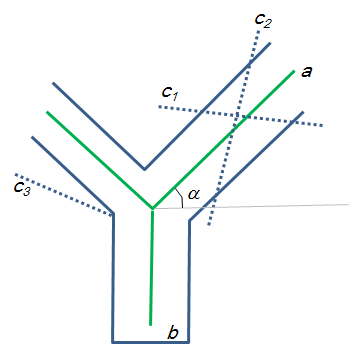
\includegraphics[width=0.3\textwidth]{figs/nonbasecut.png}
  \caption{\label{fig:nonbasecut}%
           Proof of Lemma 1: The red lines indicate the skeletons, the dashed lines indicate the cuts.}
\end{figure}

Each arc of $H_i$ subtends to the horizon by an angle of no smaller than $\pi/2 - \theta$. Let $c$ be a facet left on $M_i$ that has an outward pointing normal $n(c)$, if $n(c)$ points upwards, then $c$ is supported by the material of $M_i$ beneath it (e.g., cut $c_1$ in Figure \ref{fig:nonbasecut}); on the other hand, $n(c)$ points downwards. In the latter case, let $a$ be the arc of the skeleton that $c$ cuts through, $a$ subtends to the horizon by an angle of $\alpha \geq  \pi/2 - \theta$, $c$ must subtend to the horizon by an angle of larger than $\alpha$, and therefore greater than $\pi/2 - \theta$, which means that $c$ is support free (e.g., cut $c_2$ in Figure \ref{fig:nonbasecut}).
Hence, $c$ requires support if and only if its outward pointing normal $n(c)$ is directed downward and $n(c)$ subtends to the horizon by an angle of smaller than $\pi/2 - \theta$. But his means that $c$ cannot cut through the interior of $M_i$ (e.g., cut $c_3$ in Figure \ref{fig:nonbasecut}), this is a contradiction and completes the proof. \qed }}



In order to determine whether a cutting plane cuts through any subgraph other than $H_i$, we take advantage of the correspondence between the mesh vertices and the skeleton nodes. Since each vertex of $M$ is mapped to a single node of $S$ \cite{AuTCCL08}, as a cut goes through the mesh surface, the endpoints of the edges of $M$ that are intersected give us the information of the potential subgraph that is cut through. Approximately, if a cut $c$ goes into an edge whose endpoints are incident to a subgraph $H_j$, then $c$ cuts through $H_j$.
%On the other hand, if $v$ is an internal node to at least two subgraphs, see Figure \ref{fig:cross}, then a partition of one subgraph around $v$ is inevitable. The partition scheme follows from the operations on the fillets.

Sometimes, it is possible that a mesh component is not printable free of support even though its corresponding skeleton is printable free of support. This is because the skeleton piece that shares a junction node with some other subgraph may compromise its topology locally \cite{AuTCCL08}, and therefore cannot precisely describe the local topology feature of the partitioned component. In this case, we search along the skeleton and further partition it with an additional cut. Refer to Figure \ref{fig:arm} for an illustration. Empirically, we found this rarely happened.

\begin{figure}[tbp]
  \centering
  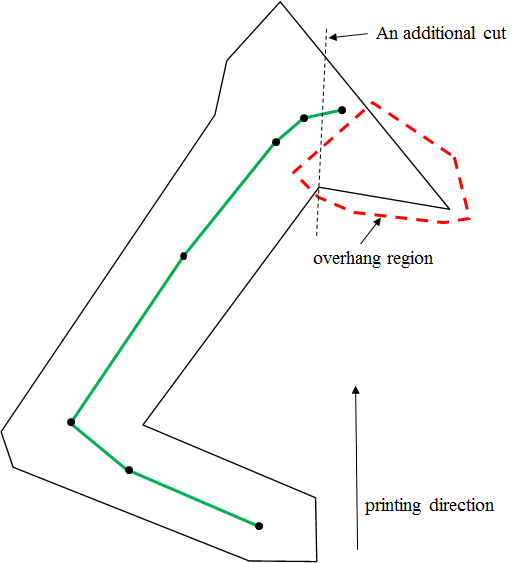
\includegraphics[width=0.3\textwidth]{figs/arm.png}
  \caption{\label{fig:arm}%
           Illustration of a mesh component with an overhange that requires support while its corresponding skeleton is support-free}
\end{figure}

%Finally, if the cut-subgraph constraint (Eq. (5)) is violated, a sequence of iterative cutting is required.








